
%(BEGIN_QUESTION)
% Copyright 2008, Tony R. Kuphaldt, released under the Creative Commons Attribution License (v 1.0)
% This means you may do almost anything with this work of mine, so long as you give me proper credit

The Rockwell/Allen-Bradley MicroLogix 1000 programmable logic controller (PLC) can handle up to four analog input signals: two with a 0-10 V maximum range and two with a 0-20 mA maximum signal range.  This PLC's analog input terminal block looks like this (the internal resistors are shown inside the PLC box):

$$\includegraphics[width=15.5cm]{i03253x01.eps}$$

Sketch the appropriate wiring to connect a pair of 4-20 mA loop-powered transmitters to the two voltage inputs (IA/0 and IA/1) on the PLC.  Sketch precision resistors in the appropriate locations to convert the 4-20 mA current signals into 1-5 V voltage signals appropriate for those input channels.

\vfil 

Note: the two ``IA SHD'' terminals are provided for cable shield conductor attachment.  You may ignore cable shield wires and these terminals for simplicity's sake.

\underbar{file i03253}
\eject
%(END_QUESTION)





%(BEGIN_ANSWER)

This is a graded question -- no answers or hints given!
 
%(END_ANSWER)





%(BEGIN_NOTES)

This is just one possible solution:

$$\includegraphics[width=15.5cm]{i03253x02.eps}$$

A general principle to apply here is that a voltage-sensing instrument input should be regarded in the same way that a voltmeter is: to be connected across the voltage to be measured.  First, identify the two terminals for each ``voltmeter'' inside the PLC (IA/0 V(+) and IA ($-$) for channel 0; IA/1 V(+) and IA ($-$) for channel 1.  Then, connect appropriate loop resistances across these terminal pairs so the PLC will sense the voltage across each resistor, and finally sketch the circuit wiring so that each transmitter's 4-20 mA current will flow through its respective resistor.

Incidentally, the exact resistor value necessary to obtain a {\it total} resistance of 250 $\Omega$ at the PLC inputs is 250.3 $\Omega$, taking into account the 210 k$\Omega$ input impedance of each voltage input channel.  However, if you were to use a 250.0 ohm resistor, it would still be possible to scale the measurement inside the PLC's programming to correct for the (slightly) incorrect equivalent loop resistance value.

%INDEX% Pictorial circuit review (4-20 mA loop)

%(END_NOTES)


